\documentclass{beamer}

\usepackage[ruled]{algorithm2e}
\SetKw{KwRet}{return}
\usepackage{amsmath}

\usetheme{AnnArbor}
\usecolortheme{crane}
\usefonttheme[onlymath]{serif}

\title{Deep Learning - Foundations and Concepts}
\subtitle{Chapter 12. Transformers}
\author{nonlineark@github}
\date{\today}

\begin{document}

\begin{frame}
    \titlepage
\end{frame}

\begin{frame}
    \frametitle{Outline}
    \tableofcontents
\end{frame}

\section{Attention}

\begin{frame}
    \frametitle{Attention}
    The fundamental concept that underpins a transformer is attention:
    \begin{itemize}
        \item This was originally developed as an enhancement to RNNs for machine translation (\href{https://arxiv.org/abs/1409.0473}{Bahdanau, Cho and Bengio, 2014})
        \item Later, it was found that significantly improved performance could be obtained by eliminating the recurrence structure and instead focusing exclusively on the attention mechanism (\href{https://arxiv.org/abs/1706.03762}{Vaswani et al., 2017}).
    \end{itemize}
\end{frame}

\begin{frame}
    \frametitle{Attention}
    Consider the following two sentences:
    \begin{itemize}
        \item I swam across the river to get to the other bank.
        \item I walked across the road to get cash from the bank.
    \end{itemize}
    Here the word ``bank'' has different meanings in the two sentences:
    \begin{itemize}
        \item In the first sentence, the words ``swam'' and ``river'' most strongly indicate that ``bank'' refers to the side of a river.
        \item In the second sentence, the word ``cash'' is a strong indicator that ``bank'' refers to a financial institution.
    \end{itemize}
    To determine the appropriate interpretation of ``bank'', a neural network processing such a sentence should:
    \begin{itemize}
        \item Attend to specific words from the rest of the sequence.
        \item The particular locations that should receive more attention depend on the input sequence itself.
    \end{itemize}
\end{frame}

\begin{frame}
    \frametitle{Transformer processing}
    \begin{itemize}
        \item The input data to a transformer is a set of vectors $\{x_{n}\}$ of dimensionality $D$, where $n=1,\hdots,N$.
        \item We refer to these data vectors as tokens, and the elements of the tokens are called features.
        \item We will combine the tokens into a matrix $X$ of dimension $N\times{}D$ in which the $n$th row comprises the token $x_{n}^{T}$.
    \end{itemize}
    \begin{figure}
        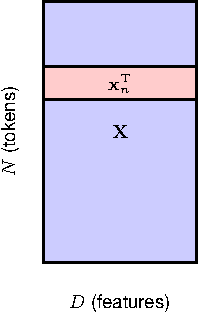
\includegraphics[height=0.4\textheight]{Figure_3.pdf}
    \end{figure}
\end{frame}

\begin{frame}
    \frametitle{Transformer processing}
    The fundamental building block of a transformer is a function that takes a data matrix $X$ as input and creates a transformed matrix $\tilde{X}$ of the same dimensionality as the output:
    \begin{equation*}
        \tilde{X}=\mathrm{TransformerLayer}(X)
    \end{equation*}
    A single transformer layer itself comprises two stages:
    \begin{itemize}
        \item The first stage, which implements the attention mechanism, mixes together the corresponding features from different tokens across the columns of the data matrix.
        \item The second stage acts on each row independently and transforms the features within each token.
    \end{itemize}
\end{frame}

\begin{frame}
    \frametitle{Attention coefficients}
    Suppose we have a set of input tokens $x_{1},\hdots,x_{N}$ and we want to map this set to another set $y_{1},\hdots,y_{N}$:
    \begin{itemize}
        \item $y_{n}$ should depend on all the tokens $x_{1},\hdots,x_{N}$.
        \item This dependence should be stronger for those tokens $x_{m}$ that are particularly important for determining the modified representation of $y_{n}$.
    \end{itemize}
    A simple way to achieve this is to define each output token $y_{n}$ to be a linear combination of the input tokens:
    \begin{align*}
        y_{n}&=\sum_{m=1}^{N}a_{nm}x_{m} \\
        a_{nm}&\ge{}0\qquad\sum_{m=1}^{N}a_{nm}=1
    \end{align*}
\end{frame}

\begin{frame}
    \frametitle{Self-attention}
    The problem of determining the attention coefficients can be viewed from an information retrieval perspective:
    \begin{itemize}
        \item We could view the vector $x_{n}$ as:
        \begin{itemize}
            \item The key for input token $n$.
            \item The value for input token $n$.
            \item The query for output token $n$.
        \end{itemize}
        \item To measure the similarity between the query $x_{n}$ and the key $x_{m}$, we could use their dot product: $x_{n}^{T}x_{m}$.
        \item To make sure the attention coefficients define a partition of unity, we could use the $\mathrm{softmax}$ function to transform the dot products.
    \end{itemize}
\end{frame}

\begin{frame}
    \frametitle{Self-attention}
    Dot-product self-attention:
    \begin{align*}
        y_{n}&=\sum_{m=1}^{N}a_{nm}x_{m} \\
        a_{nm}&=\frac{\exp(x_{n}^{T}x_{m})}{\sum_{m'=1}^{N}\exp(x_{n}^{T}x_{m'})}
    \end{align*}
    Or write in matrix notation:
    \begin{equation*}
        Y=\mathrm{softmax}(XX^{T})X
    \end{equation*}
    where $\mathrm{softmax}(L)$ means to apply $\mathrm{softmax}$ to each row of the matrix $L$.
\end{frame}

\begin{frame}
    \frametitle{Network parameters}
    The current transformation from input tokens $\{x_{n}\}$ to output tokens $\{y_{n}\}$ has major limitations:
    \begin{itemize}
        \item The transformation is fixed and has no capacity to learn from data because it has no adjustable parameters.
        \item Each of the feature values within a token $x_{n}$ plays an equal role in determining the attention coefficients.
    \end{itemize}
\end{frame}

\begin{frame}
    \frametitle{Network parameters}
    We can overcome these limitations by defining separate query, key and value matrices each having their own independent linear transformations:
    \begin{itemize}
        \item $Q=XW^{(q)}$, where $W^{(q)}$ has dimensionality $N\times{}D_{k}$.
        \item $K=XW^{(k)}$, where $W^{(k)}$ has dimensionality $N\times{}D_{k}$.
        \item $V=XW^{(v)}$, where $W^{(v)}$ has dimensionality $N\times{}D_{v}$.
        \item A typical choice is $D_{k}=D$.
        \item If we set $D_{v}=D$:
        \begin{itemize}
            \item This will facilitate the inclusion of residual connections.
            \item Multiple transformer layers can be stacked on top of each other.
        \end{itemize}
    \end{itemize}
    The dot-product self-attention now takes the form:
    \begin{equation*}
        Y=\mathrm{softmax}(QK^{T})V
    \end{equation*}
\end{frame}

\begin{frame}
    \frametitle{Scaled self-attention}
    \begin{itemize}
        \item When logits are too large, the $\mathrm{softmax}$ function will produce extremely small gradients, which is not desirable.
        \item We need to scale the logits before applying the $\mathrm{softmax}$ function.
        \item Notice that if $q,k\in\mathbb{R}^{D_{k}}$ and the elements of $q$ and $k$ are all independent random numbers with zero mean and unit variance, then $\mathrm{var}(q^{T}k)=D_{k}$. Thus it would be appropriate to scale the logits by the standard deviation $\sqrt{D_{k}}$.
    \end{itemize}
    The scaled dot-product self-attention now takes the form:
    \begin{equation*}
        Y=\mathrm{Attention}(Q,K,V)=\mathrm{softmax}(\frac{QK^{T}}{\sqrt{D_{k}}})V
    \end{equation*}
\end{frame}

\begin{frame}
    \frametitle{Scaled self-attention}
    \begin{figure}
        \caption{Information flow in a scaled dot-product self-attention neural network layer}
        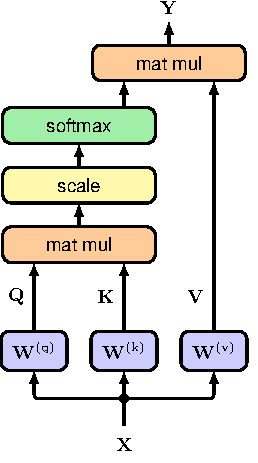
\includegraphics[height=0.7\textheight]{Figure_6.pdf}
    \end{figure}
\end{frame}

\begin{frame}
    \frametitle{Scaled self-attention}
    \begin{algorithm}[H]
        \caption{Scaled dot-product self-attention}
        $Q\gets{}XW^{(q)}$\;
        $K\gets{}XW^{(k)}$\;
        $V\gets{}XW^{(v)}$\;
        \Return{$\mathrm{Attention}(Q,K,V)=\mathrm{softmax}(\frac{QK^{T}}{\sqrt{D_{k}}})V$}\;
    \end{algorithm}
\end{frame}

\begin{frame}
    \frametitle{Multi-head attention}
    We can use multiple attention heads in parallel to attend to multiple data-dependent patterns at the same time. Suppose we have $C$ heads:
    \begin{align*}
        H_{c}&=\mathrm{Attention}(Q_{c},K_{c},V_{c}) \\
        &=\mathrm{Attention}(XW^{(q)}_{c},XW^{(k)}_{c},XW^{(v)}_{c})
    \end{align*}
    The heads are first concatenated into a single matrix, and the result is then linearly transformed using a matrix $W^{(o)}$ to give a combined output:
    \begin{equation*}
        Y=(H_{1},\hdots,H_{C})W^{(o)}
    \end{equation*}
    The matrix $W^{(o)}$ has dimension $HD_{v}\times{}D$, so that the final output matrix $Y$ has dimension $N\times{}D$.
\end{frame}

\begin{frame}
    \frametitle{Multi-head attention}
    \begin{figure}
        \caption{Information flow in a multi-head attention layer}
        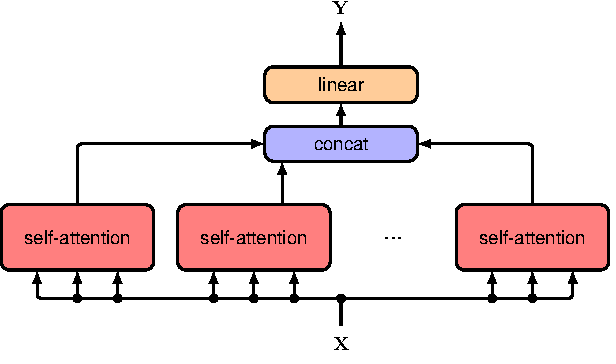
\includegraphics[height=0.7\textheight]{Figure_8.pdf}
    \end{figure}
\end{frame}

\begin{frame}
    \frametitle{Multi-head attention}
    \begin{algorithm}[H]
        \caption{Multi-head attention}
        \For{$c\gets{}1$ \KwTo $C$}{
            $Q_{c}=XW^{(q)}_{c}$\;
            $K_{c}=XW^{(k)}_{c}$\;
            $V_{c}=XW^{(v)}_{c}$\;
            $H_{c}=\mathrm{Attention}(Q_{c},K_{c},V_{c})$\;
        }
        $H=(H_{1},\hdots,H_{C})$\;
        \Return{$Y=HW^{(o)}$}\;
    \end{algorithm}
\end{frame}

\begin{frame}
    \frametitle{Transformer layers}
    To improve training efficiency, we can introduce residual connections and layer normalization:
    \begin{equation*}
        Z=\mathrm{LayerNorm}(Y(X)+X)
    \end{equation*}
    Or using pre-norm:
    \begin{equation*}
        Z=Y(\mathrm{LayerNorm}(X))+X
    \end{equation*}
    Until now, the output data matrix $Y$ is still a linear transformation of the input data matrix $X$, and this limits the expressive capabilities of the attention layer. We can enhance the flexibility by post-processing the outputs using a standard nonlinear neural network denoted $\mathrm{MLP}$:
    \begin{equation*}
        \tilde{X}=\mathrm{LayerNorm}(\mathrm{MLP}(Z)+Z)
    \end{equation*}
    Again, we can use a pre-norm instead:
    \begin{equation*}
        \tilde{X}=\mathrm{MLP}(\mathrm{LayerNorm}(Z))+Z
    \end{equation*}
\end{frame}

\begin{frame}
    \frametitle{Transformer layers}
    \begin{figure}
        \caption{One layer of the transformer architecture}
        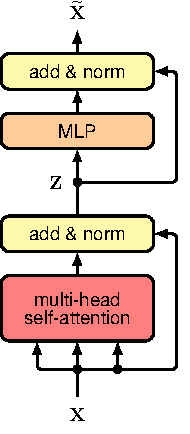
\includegraphics[height=0.7\textheight]{Figure_9.pdf}
    \end{figure}
\end{frame}

\begin{frame}
    \frametitle{Computational complexity}
    \begin{itemize}
        \item In the attention layer:
        \begin{itemize}
            \item Calculate the matrices $Q$, $K$ and $V$: $\mathcal{O}(ND^{2})$.
            \item Calculate the dot products $QK^{T}$: $\mathcal{O}(N^{2}D)$.
            \item Calculate the matrix $Y$: $\mathcal{O}(N^{2}D)$.
        \end{itemize}
        \item In the neural network layer:
        \begin{itemize}
            \item Calculate the matrix $\tilde{X}$: $\mathcal{O}(ND^{2})$.
        \end{itemize}
    \end{itemize}
\end{frame}

\begin{frame}
    \frametitle{Positional encoding}
    \begin{itemize}
        \item A transformer is equivariant with respect to input permutations due to the shared matrices $W^{(q)}_{c}$, $W^{(k)}_{c}$, $W^{(v)}_{c}$ and the shared subsequent neural network.
        \item The lack of dependence on token order becomes a major limitation when we consider sequential data, so we need to find a way to inject token order information into the network.
    \end{itemize}
\end{frame}

\begin{frame}
    \frametitle{Positional encoding}
    The requirements for a positional encoding:
    \begin{itemize}
        \item The token order should be encoded in the data itself instead of having to be represented in the network architecture.
        \item We will construct a position encoding vector $r_{n}$ associated with each input position $n$ and then combine this with the associated input token $x_{n}$:
        \begin{itemize}
            \item {[No]} $\tilde{x}_{n}=(x_{n},r_{n})$.
            \item {[Yes]} $\tilde{x}_{n}=x_{n}+r_{n}$.
        \end{itemize}
        \item $r_{n}$ should be bounded.
        \item $r_{n}$ should generalize well to new input sequences that are longer than those used in training.
        \item $r_{n}$ should be unique for a given position.
        \item $r_{n}$ should have a consistent way to express the number of steps between any two input tokens irrespective of their absolute position.
    \end{itemize}
\end{frame}

\begin{frame}
    \frametitle{Positional encoding}
    Positional encoding based on sinusoidal functions:
    \begin{align*}
        r_{ni}=\begin{cases}
            \sin(\frac{n}{L^{\frac{i}{D}}}),\textrm{if $i$ is even} \\
            \cos(\frac{n}{L^{\frac{i-1}{D}}}),\textrm{if $i$ is odd}
        \end{cases}
    \end{align*}
    \begin{figure}
        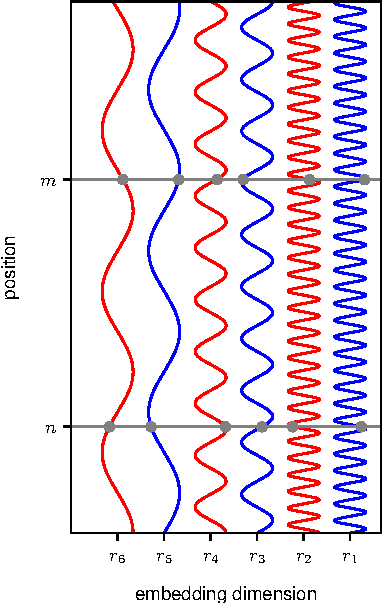
\includegraphics[height=0.5\textheight]{Figure_10_a.pdf}
    \end{figure}
\end{frame}

\section{Natural Language}

\begin{frame}
    \frametitle{Word embedding}
    To convert the words into a numerical representation that is suitable for use as the input to a deep neural network:
    \begin{itemize}
        \item {[No]} One simple approach is to define a fixed dictionary of words, and use a one hot representation for each word.
        \item The embedding process can be defined by a matrix $E$ of size $D\times{}K$ where $D$ is the dimensionality of the embedding space and $K$ is the dimensionality of the dictionary. Each column of $E$ represents the embedding of a word.
    \end{itemize}
\end{frame}

\begin{frame}
    \frametitle{Word embedding}
    The word2vec technique:
    \begin{itemize}
        \item A training set is constructed in which each sample is obtained by considering a window of $M$ adjacent words in the text, where a typical value might be $M=5$.
        \item The error function is defined as the sum of the error functions for each sample.
        \item In continuous bag of words, the target variable for network training is the middle word, and the remaining context words form the inputs.
        \begin{itemize}
            \item Once trained, $E$ is given by the transpose of the second-layer weight matrix.
        \end{itemize}
        \item In skip-grams, the center word is presented as the input and the target values are the context words.
        \begin{itemize}
            \item Once trained, $E$ is given by the first-layer weight matrix.
        \end{itemize}
    \end{itemize}
\end{frame}

\begin{frame}
    \frametitle{Word embedding}
    \begin{figure}
        \caption{Two-layer neural networks used to learn word embeddings}
        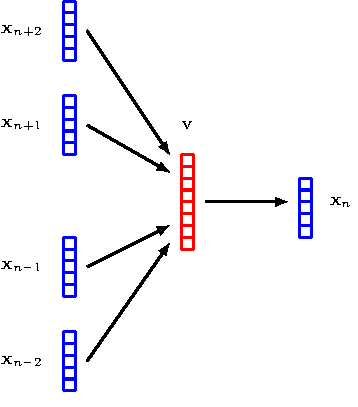
\includegraphics[width=0.4\textwidth]{Figure_11_a.pdf}
        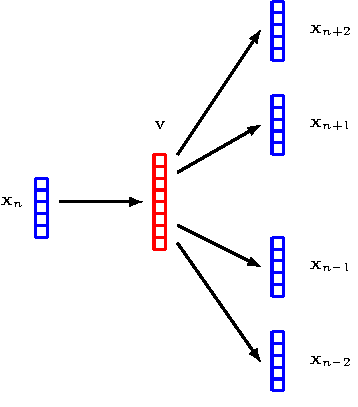
\includegraphics[width=0.4\textwidth]{Figure_11_b.pdf}
    \end{figure}
\end{frame}

\begin{frame}
    \frametitle{Word embedding}
    Words that are semantically related are mapped to nearby positions in the embedding space.
    \bigbreak
    The learned embedding space often has an even richer semantic structure than just the proximity of related words, and that this allows for simple vector arithmetic:
    \begin{equation*}
        v(\textrm{Paris})-v(\textrm{France})\approx{}v(\textrm{Rome})-v(\textrm{Italy})
    \end{equation*}
\end{frame}

\begin{frame}
    \frametitle{Tokenization}
    \begin{itemize}
        \item Limitations in word-level representation:
        \begin{itemize}
            \item Words not in the dictionary.
            \item Misspelled words.
            \item Punctuation symbols or other character sequences such as computer code.
        \end{itemize}
        \item Limitations in character-level representation:
        \begin{itemize}
            \item The semantically important word structure of language is discarded.
            \item Requires a much larger number of sequential steps for a given body of text, thereby increasing the computational cost of processing the sequence.
        \end{itemize}
        \item We can combine the benefits of character-level and word-level representations by using a pre-processing step that converts a string of words and punctuation symbols into a string of tokens.
    \end{itemize}
\end{frame}

\begin{frame}
    \frametitle{Tokenization}
    \begin{figure}
        \caption{Tokenizing natural language by analogy with byte pair encoding}
        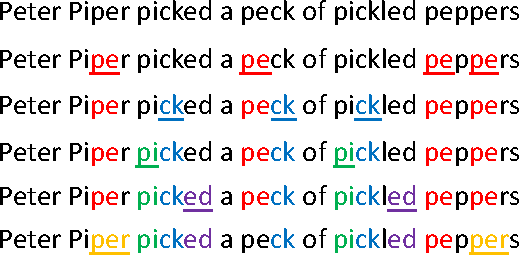
\includegraphics{Figure_12.pdf}
    \end{figure}
\end{frame}

\begin{frame}
    \frametitle{Bag of words}
    The bag-of-words model assumes that the words are drawn independently from the same distribution and hence that the joint distribution is fully factorized in the form:
    \begin{equation*}
        p(x_{1},\hdots,x_{N})=\prod_{n=1}^{N}p(x_{n})
    \end{equation*}
    The bag-or-words model completely ignores the ordering of the words.
\end{frame}

\begin{frame}
    \frametitle{Autoregressive models}
    The autoregressive approach assumes that each of the conditional distributions is independent of all previous observations except the $L$ most recent words. For example, for $L=2$:
    \begin{equation*}
        p(x_{1},\hdots,x_{N})=p(x_{1})p(x_{2}|x_{1})\prod_{n=3}^{N}p(x_{n}|x_{n-1},x_{n-2})
    \end{equation*}
    The case with $L=1$ is known as a bi-gram model; when $L=2$, it is called a tri-gram model; and in general these are called n-gram models.
\end{frame}

\begin{frame}
    \frametitle{Recurrent neural networks}
    \begin{figure}
        \caption{A general RNN with parameters $w$}
        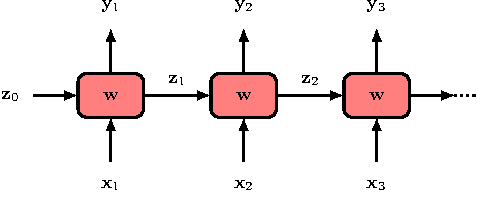
\includegraphics{Figure_13.pdf}
    \end{figure}
\end{frame}

\begin{frame}
    \frametitle{Recurrent neural networks}
    \begin{figure}
        \caption{An example of a recurrent neural network used for language translation}
        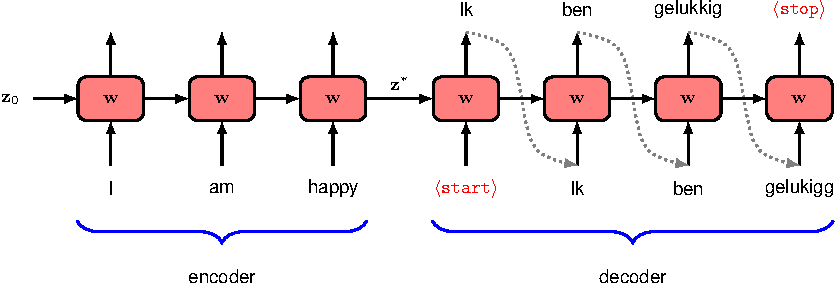
\includegraphics[width=0.8\textwidth]{Figure_14.pdf}
    \end{figure}
\end{frame}

\begin{frame}
    \frametitle{Backpropagation through time}
    \begin{itemize}
        \item RNNs can be trained by stochastic gradient descent. The error function consists of a sum over all output units of the error for each unit, in which each output unit has a $\mathrm{softmax}$ activation function along with an associated cross-entropy error function.
        \begin{itemize}
            \item In practice, for very long sequences, training can be difficult due to the problems of vanishing gradients or exploding gradients.
        \end{itemize}
        \item Bottleneck problem: RNNs deal poorly with long-range dependencies. For the translation task, the entire concept of the English sentence must be captured in the single hidden vector $z^{*}$ of fixed length, which becomes increasingly problematic with longer sequences.
        \item RNNs do not support parallel computation within a single training example due to the sequential nature of the processing.
    \end{itemize}
\end{frame}

\section{Transformer Language Models}

\begin{frame}
    \frametitle{Transformer language models}
    Transformers can be applied to many different kinds of language processing task, and can be grouped into three categories:
    \begin{itemize}
        \item Encoder. For example, sentiment analysis, in which we take a sequence of words as input and provide a single variable representing the sentiment of the text.
        \item Decoder. For example, image caption generation, in which we take a single image as input and generate a word sequence as output.
        \item Sequence-to-sequence. For example, machine translation, in which both the input and output comprise a sequence of words.
    \end{itemize}
\end{frame}

\begin{frame}
    \frametitle{Decoder transformers}
    \begin{figure}
        \caption{Architecture of a GPT decoder transformer network}
        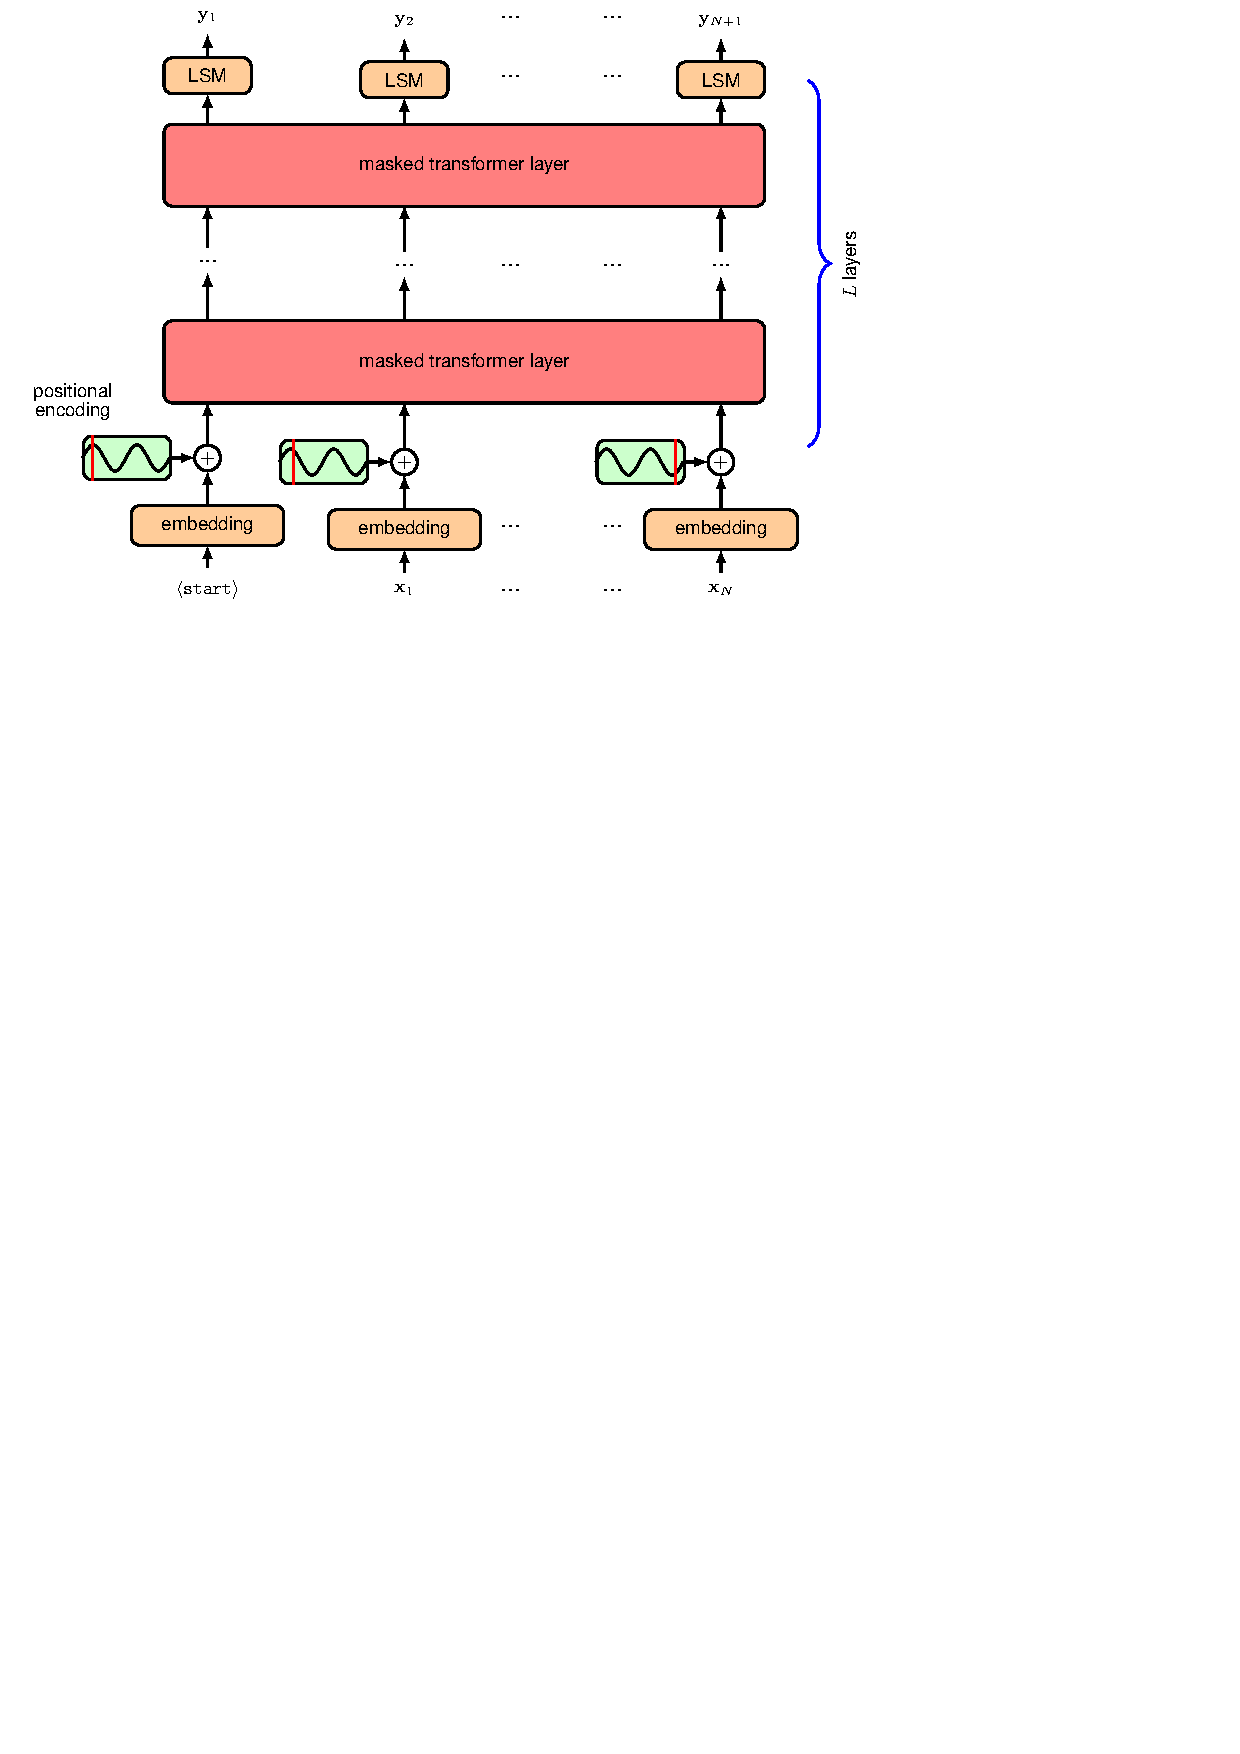
\includegraphics[trim=0 16cm 0 0,clip=true,width=0.8\textwidth]{Figure_15.pdf}
    \end{figure}
\end{frame}

\begin{frame}
    \frametitle{Decoder transformers}
    \begin{itemize}
        \item The stack of transformer layers take a sequence $x_{1},\hdots,x_{N}$ of tokens, each of dimensionality $D$, as input and produce a sequence $\tilde{x}_{1},\hdots,\tilde{x}_{N}$ of tokens, again of dimensionality $D$, as output.
        \item We make a linear transformation of each output token using a matrix $W^{(p)}$ of dimensionality $D\times{}K$ followed by a $\mathrm{softmax}$ activation function so that each output represents a probability distribution over the dictionary of tokens: $Y=\mathrm{softmax}(\tilde{X}W^{(p)})$.
        \item Each $\mathrm{softmax}$ output unit has an associated cross-entropy error function, and the error function used for training is the sum of the cross-entropy error values summed over the training set.
    \end{itemize}
\end{frame}

\begin{frame}
    \frametitle{Decoder transformers}
    \begin{itemize}
        \item We can achieve much greater efficiency by processing an entire sequence at once so that each token acts both as a target value for the sequence of previous tokens and as an input value for subsequent tokens.
        \item However, we have to ensure that the network is not able to cheat by looking ahead in the sequence:
        \begin{itemize}
            \item We shift the input sequence to the right by one step.
            \item We introduce masked attention into each of the attention layers, in which we set to zero all of the attention weights that correspond to a token attending to any later token in the sequence.
        \end{itemize}
    \end{itemize}
\end{frame}

\begin{frame}
    \frametitle{Decoder transformers}
    \begin{figure}
        \caption{An illustration of the mask matrix for masked self-attention}
        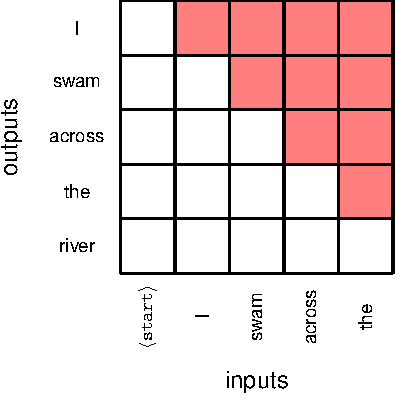
\includegraphics[height=0.7\textheight]{Figure_16.pdf}
    \end{figure}
\end{frame}

\begin{frame}
    \frametitle{Decoder transformers}
    \begin{itemize}
        \item To make efficient use of the massive parallelism of GPUs, multiple sequences may be stacked together into an input tensor for parallel processing in a single batch.
        \item The sequences are padded to the same length by introducing a specific token {\tt <pad>}.
        \item An additional mask is then used in the attention weights to ensure that the outputs do not pay attention to any inputs occupied by the {\tt <pad>} token.
    \end{itemize}
\end{frame}

\begin{frame}
    \frametitle{Sampling strategies}
    There are several options for selecting the value of the token based on the computed probabilities:
    \begin{itemize}
        \item One extreme is greedy search, which simply selects the token with the highest probability.
        \begin{itemize}
            \item Deterministic, $\mathcal{O}(KN)$ cost, far from optimal.
        \end{itemize}
        \item The other extreme is exhaustive search, which enumerates all the possible output sequences and then outputs the one that scores the highest predicted probability.
        \begin{itemize}
            \item Infeasible given the total number of sequences is $K^{N}$.
        \end{itemize}
    \end{itemize}
\end{frame}

\begin{frame}
    \frametitle{Sampling strategies}
    Beam search:
    \begin{itemize}
        \item At each step, we maintain a set of $B$ hypotheses, where $B$ is called the beam width.
        \item We then feed all these sequences through the network, and for each sequence we find the $B$ most probable token values, thereby creating $B^{2}$ possible hypotheses for the extended sequence.
        \item This list is then pruned by selecting the most probable $B$ hypotheses.
        \item The sequence probabilities are generally normalized by the corresponding lengths of the sequence before making comparisons to prevent bias towards short sequences.
        \item Beam search has cost $\mathcal{O}(BKN)$.
    \end{itemize}
\end{frame}

\begin{frame}
    \frametitle{Sampling strategies}
    \begin{itemize}
        \item One problem with approaches such as greedy search and beam search is that they limit the diversity of potential outputs.
        \item Top-$K$ sampling: Consider only the states having the top $K$ probabilities, for some choice of $K$, and then sample from these according to their renormalized probabilities.
        \item Top-$p$ sampling: Calculates the cumulative probability of the top outputs until a threshold is reached and then samples from this restricted set of token states.
    \end{itemize}
\end{frame}

\begin{frame}
    \frametitle{Sampling strategies}
    A softer version of top-$K$ sampling is to introduce a parameter $T$ called temperature into the definition of the $\mathrm{softmax}$ function: $y_{i}=\frac{\exp(\frac{a_{i}}{T})}{\sum_{j}\exp(\frac{a_{j}}{T})}$.
    \begin{itemize}
        \item When $T\to{}0$, the probability mass is concentrated on the most probable state.
        \item For $T=1$, we recover the unmodified $\mathrm{softmax}$ distribution.
        \item For $T\to\infty$, the distribution becomes uniform across all states.
        \item By choosing a value in the range $0<T<1$, the probability is concentrated towards the higher values.
    \end{itemize}
\end{frame}

\begin{frame}
    \frametitle{Encoder transformers}
    \begin{figure}
        \caption{Architecture of an encoder transformer model}
        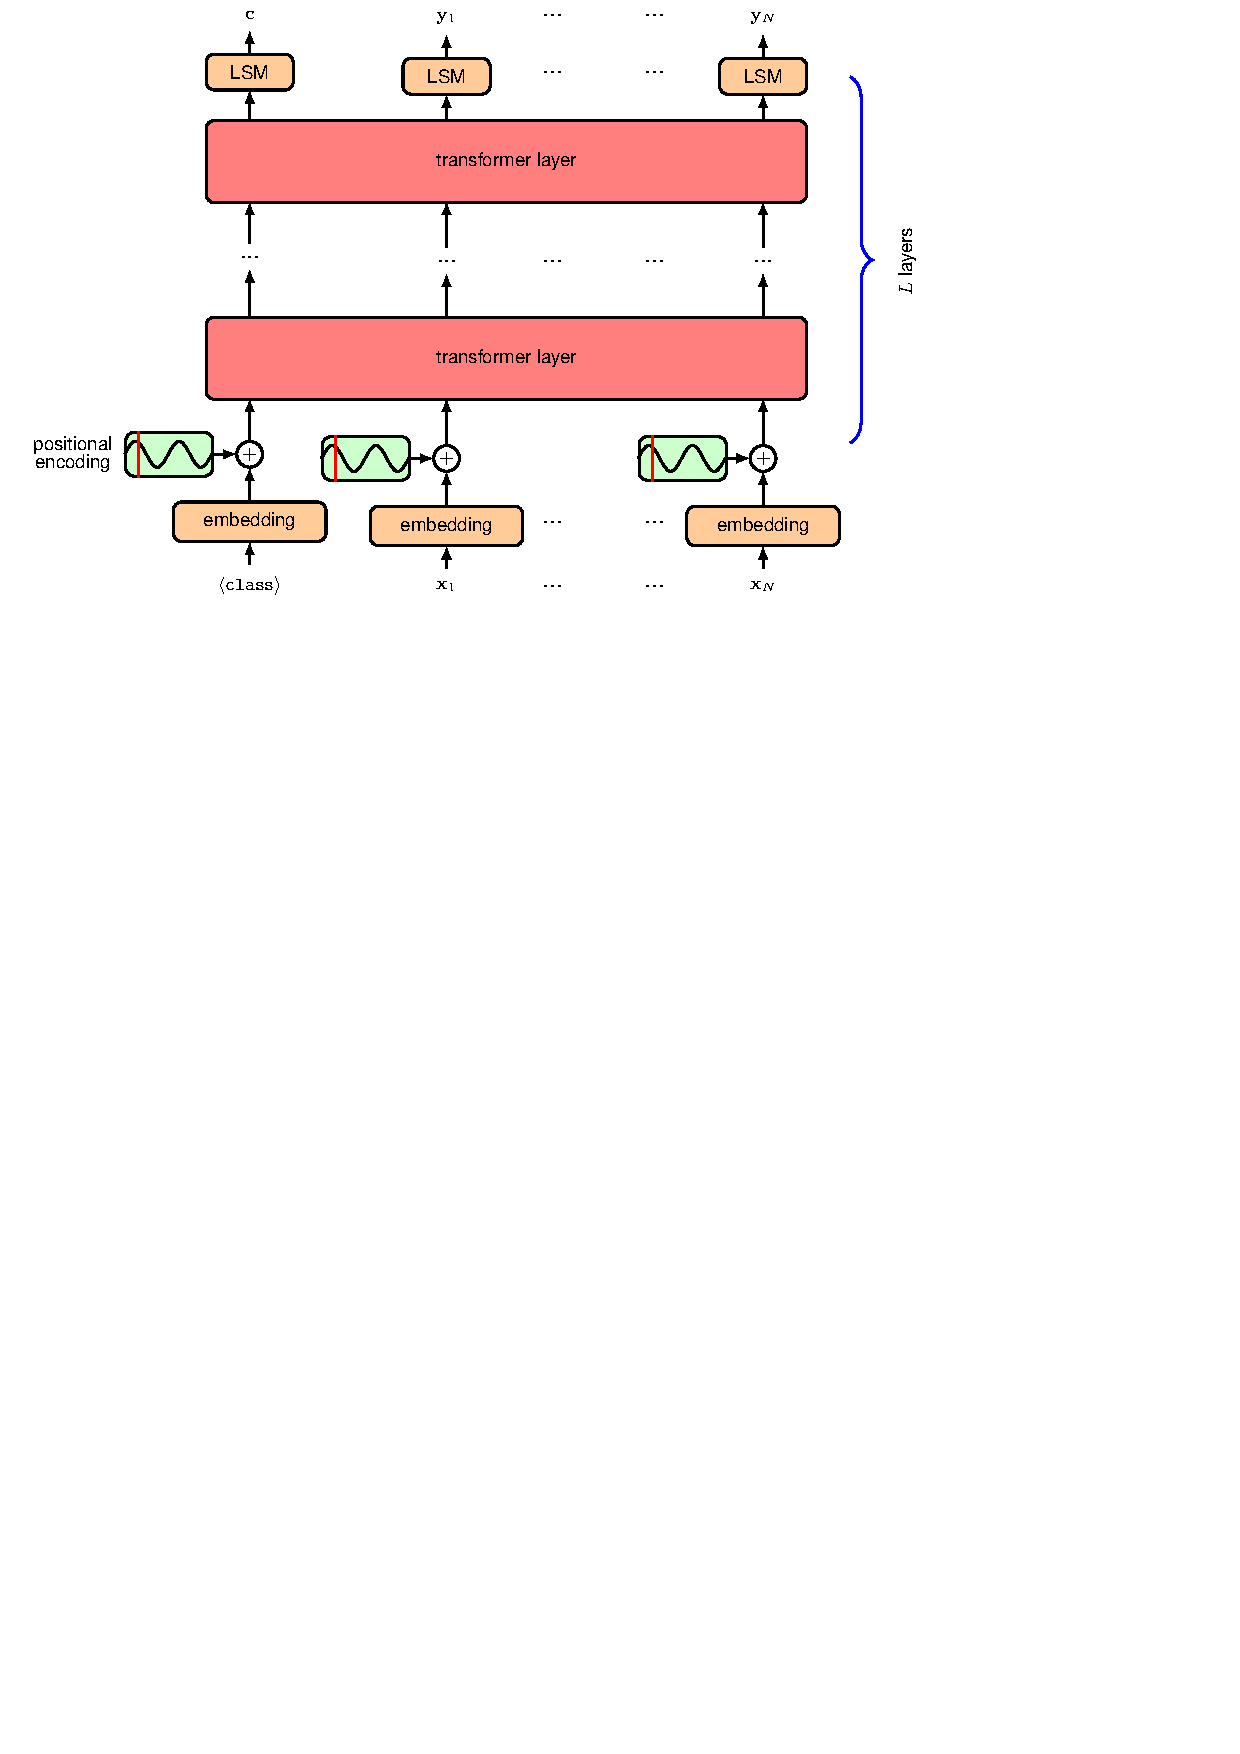
\includegraphics[trim=0 16cm 0 0,clip=true,width=0.8\textwidth]{Figure_18.pdf}
    \end{figure}
\end{frame}

\begin{frame}
    \frametitle{Encoder transformers}
    \begin{itemize}
        \item The first token of every input string is given by a special token {\tt <class>}, and the corresponding output of the model is ignored during pre-training.
        \item A randomly chosen subset of the input tokens, say $15\%$, are replaced with a special token denoted {\tt <mask>}. The model is trained to predict the missing tokens at the corresponding output nodes.
    \end{itemize}
\end{frame}

\begin{frame}
    \frametitle{Encoder transformers}
    Once the encoder model is trained it can then be fine-tuned for a variety of different tasks:
    \begin{itemize}
        \item For a text classification task, only the first output position is used, which corresponds to the {\tt <class>} token that always appears in the first position of the input sequence.
        \item If the goal is to classify each token of the input string, then the first output is ignored and the subsequent outputs have a shared linear-plus-softmax layer.
        \item Alternatively the output of a pre-trained model might feed into a sophisticated generative deep learning model for applications such as text-to-image synthesis.
    \end{itemize}
\end{frame}

\begin{frame}
    \frametitle{Sequence-to-sequence transformers}
    \begin{figure}
        \caption{Schematic illustration of one cross-attention layer}
        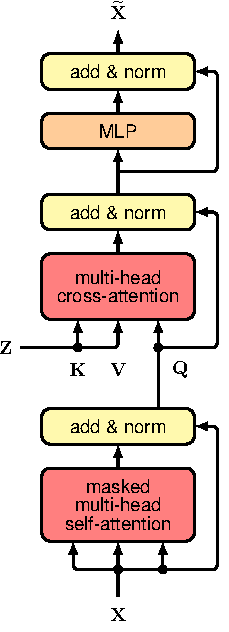
\includegraphics[height=0.7\textheight]{Figure_19.pdf}
    \end{figure}
\end{frame}

\begin{frame}
    \frametitle{Sequence-to-sequence transformers}
    \begin{itemize}
        \item An encoder transformer can be used to map the input token sequence into a suitable internal representation $Z$.
        \item Cross attention: The query vectors come from the sequence being generated, the key and value vectors come from the sequence represented by $Z$.
    \end{itemize}
\end{frame}

\begin{frame}
    \frametitle{Sequence-to-sequence transformers}
    \begin{figure}
        \caption{Schematic illustration of a sequence-to-sequence transformer}
        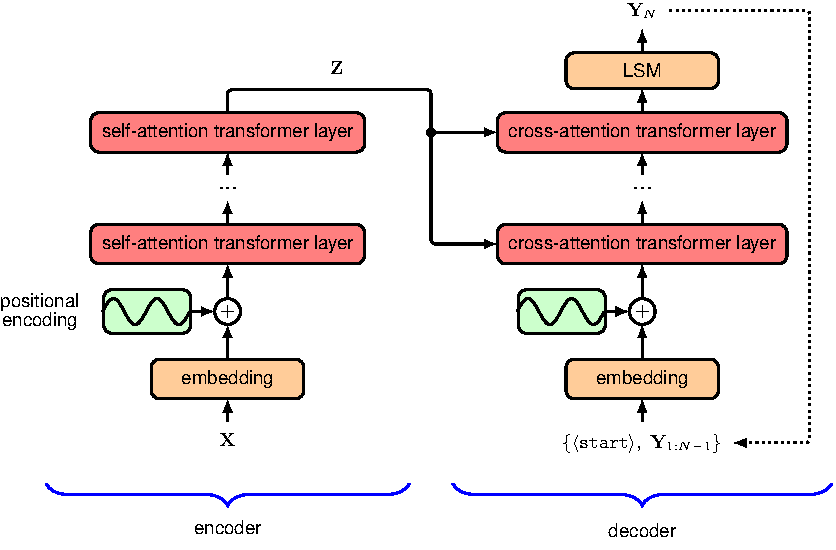
\includegraphics[width=0.8\textwidth]{Figure_20.pdf}
    \end{figure}
\end{frame}

\begin{frame}
    \frametitle{Large language models}
    \begin{itemize}
        \item The use of self-supervised learning led to a paradigm shift in which a large model is first pre-trained using unlabelled data and then subsequently fine-tuned using supervised learning based on a much smaller set of labelled data.
        \item Fine-tuning can be done by adding extra layers to the outputs of the network or by replacing the last few layers with fresh parameters and then using the labelled data to train these final layers.
    \end{itemize}
\end{frame}

\begin{frame}
    \frametitle{Large language models}
    Low-rank adaptation (LoRA):
    \begin{itemize}
        \item A trained over-parameterized model has a low intrinsic dimensionality with respect to fine-tuning.
        \item LoRA freezes the weights of the original model and adds additional learnable weight matrices into each layer of the transformer in the form of low-rank products.
        \item Typically only attention-layer weights are modified, whereas MLP-layer weights are kept fixed.
    \end{itemize}
\end{frame}

\begin{frame}
    \frametitle{Large language models}
    \begin{figure}
        \caption{Schematic illustration of low-rank adaptation}
        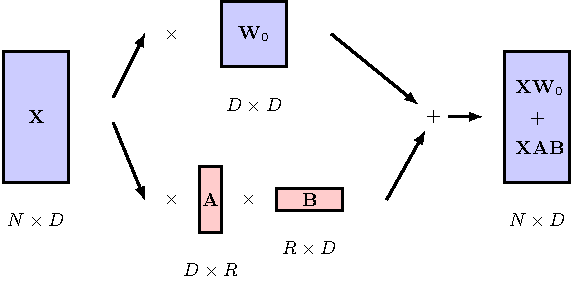
\includegraphics{Figure_21.pdf}
    \end{figure}
\end{frame}

\begin{frame}
    \frametitle{Large language models}
    \begin{itemize}
        \item As language models have become larger and more powerful, the need for fine-tuning has diminished, with generative language models now able to solve a broad range of tasks simply through text-based interaction.
        \item Reinforcement learning through human feedback (RLHF): Fune-tuning large language models through human evaluation of generated output.
        \item The performance of the model now depends on the form of the prompt, leading to a new field called prompt engineering.
        \item Few-shot learning: By providing some examples within the prompt, the model is able to solve new tasks.
    \end{itemize}
\end{frame}

\section{Multimodal Transformers}

\begin{frame}
    \frametitle{Multimodal transformers}
    \begin{itemize}
        \item Transformers have proved to be general-purpose models, and become prevalent in nearly all areas of deep learning.
        \item The core architecture of the transformer layer has remained relatively constant, both over time and across applications.
        \item The key innovations that enabled the use of transformers in areas other than natural language have largely focused on the representation and encoding of the inputs and outputs.
        \item One big advantage of a single architecture that is capable of processing many different kinds of data is that it makes multimodal computation relatively straightforward.
    \end{itemize}
\end{frame}

\begin{frame}
    \frametitle{Vision transformers}
    How to convert an input image into tokens:
    \begin{itemize}
        \item Split the image into a set of patches of the same size.
        \item Feed the image through a small convolutional neural network, which can down-sample the image to give a manageable number of tokens each represented by one of the network outputs.
    \end{itemize}
    How to encode positional information in the tokens:
    \begin{itemize}
        \item It is possible to construct explicit positional embeddings that encode the two-dimensional positional information of the image patches, but in practice this does not generally improve performance.
        \item It is most common to just use learned positional embeddings.
    \end{itemize}
\end{frame}

\begin{frame}
    \frametitle{Generative image transformers}
    \begin{itemize}
        \item Images have no natural ordering of their pixels, so it is not intuitive that decoding them autoregressively would be useful.
        \item Howerver, any distribution can be decomposed into a product of conditionals, provided we first define some ordering of the variables.
        \item One widely used choice for ordering for the pixels is called raster scan.
    \end{itemize}
    \begin{figure}
        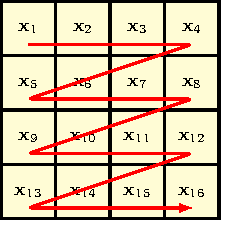
\includegraphics{Figure_23.pdf}
    \end{figure}
\end{frame}

\begin{frame}
    \frametitle{Generative image transformers}
    \begin{itemize}
        \item Continuous conditional distributions learned by maximum likelihood tend to learn averages of the training data, leading to blurry images.
        \item Much better results are obtained for image generation by using discrete representations.
        \begin{itemize}
            \item Each pixel has $2^{24}$ possible values ($8$ bits for each of the three channels), learning a conditional $\mathrm{softmax}$ distribution over such a high-dimensional space is infeasible.
            \item Vector quantization:
            \begin{itemize}
                \item Introduce a set of $K$ codebook vectors.
                \item Approximate each data vector by its nearest codebook vector according to some similarity metric.
            \end{itemize}
        \end{itemize}
    \end{itemize}
\end{frame}

\begin{frame}
    \frametitle{Generative image transformers}
    The ImageGPT model:
    \begin{itemize}
        \item Each pixel is treated as one of a discrete set of three-dimensional color codebook vectors.
        \item A one-hot encoding therefore gives discrete tokens, and allows the transformer to be trained in the same way as language models, with a next-token classification objective.
    \end{itemize}
\end{frame}

\begin{frame}
    \frametitle{Audio data}
    \begin{itemize}
        \item Sound is generally stored as a waveform.
        \item The waveform is pre-processed into mel spectrogram, which is a matrix whose columns represent time steps and whose rows correspond to frequencies.
        \item The mel spectrogram is viewed as an image which is then tokenized in a similar way to vision transformers.
    \end{itemize}
\end{frame}

\begin{frame}
    \frametitle{Text-to-speech}
    Vall-E (a neural codec language model):
    \begin{itemize}
        \item Speech data is converted into a sequence of discrete tokens from a learned dictionary or codebook obtained using vector quantization.
        \item The input:
        \begin{itemize}
            \item Text tokens from a passage of text.
            \item Additional speech tokens from a short segment of unrelated speech from the same speaker.
        \end{itemize}
        \item Target outputs for training consist of the corresponding speech tokens.
    \end{itemize}
\end{frame}

\begin{frame}
    \frametitle{Text-to-speech}
    \begin{figure}
        \caption{A diagram showing the high-level architecture of Vall-E}
        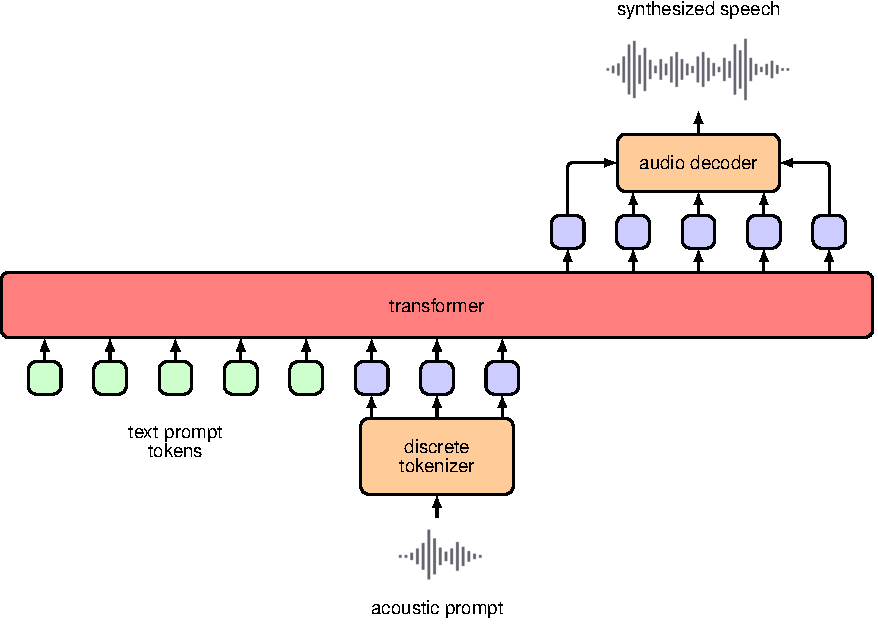
\includegraphics[height=0.7\textheight]{Figure_26.pdf}
    \end{figure}
\end{frame}

\begin{frame}
    \frametitle{Vision and language transformers}
    \begin{figure}
        \caption{Examples of the CM3Leon model performing a variety of different tasks}
        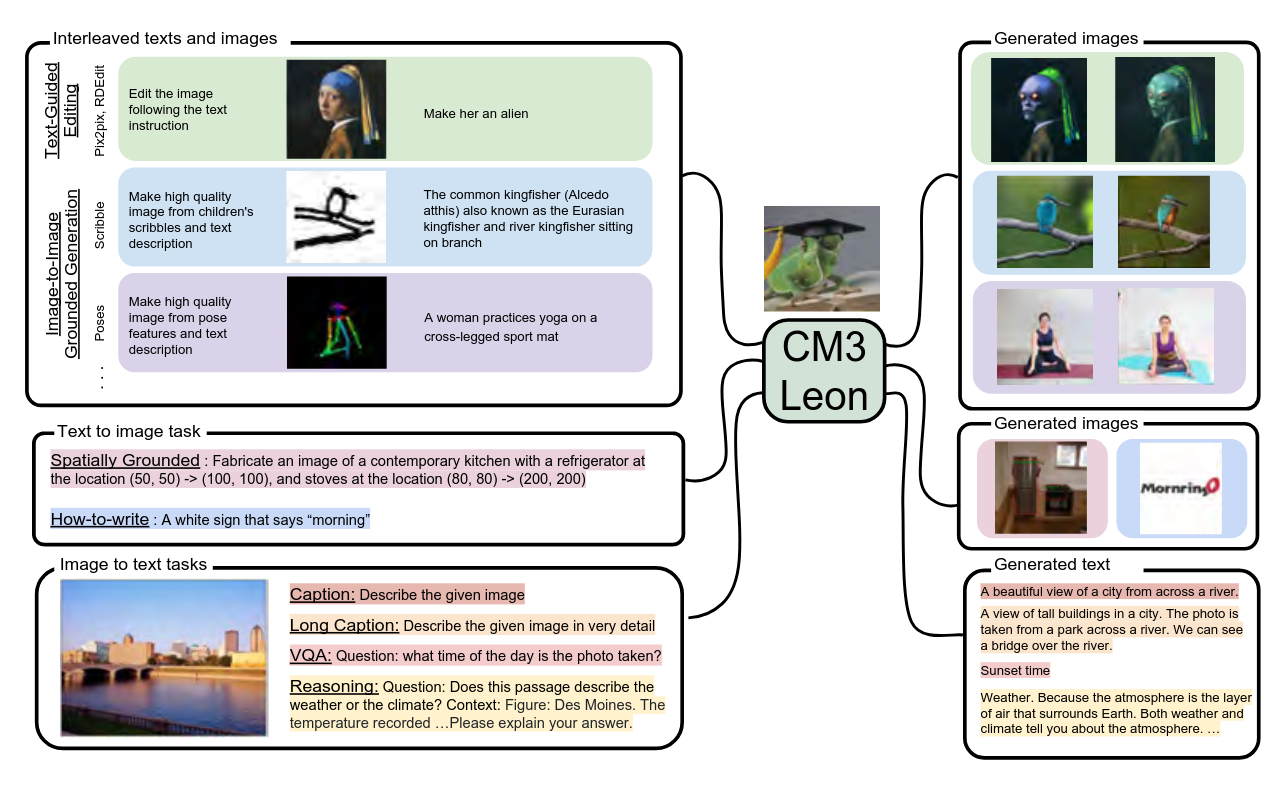
\includegraphics[width=0.8\textwidth]{Figure_27.png}
    \end{figure}
\end{frame}

\end{document}